\section{Méthode} \label{sec: method}
    L'étude et la caractérisation numérique des attracteurs chaotiques
    requiert la connaissance de plusieurs méthodes/algorithmes. L'utilisation
    du langage de \textit{haut niveau} Python est donc agréable grâce à la
    manipulation intuitive des objets mathématiques multidimensionnels et dans
    l'implémentation de diverses méthodes numériques. On explicitera ici la
    façon dont les attracteurs présentés dans la section
    \fullref{subsec: attractors} ont été simulés, comment le spectre de
    Lyapunov à été calculé et finalement l'algorithme avec lequel ce spectre a
    pu été estimé pour un temps de simulation $t\to\infty$.

\subsection{Équations différentielles} \label{subsec: res_diff}
    Les systèmes d'équations différentielles \eqref{eq : lorenz},
    \eqref{eq : rossler} et \eqref{eq : bouali} qui décrivent les attracteurs
    étudiés dans ce travail on tous pu être simulé pour des configurations
    données de l'espace des phases (ex: conditions initiales, coefficients,
    etc.). Les simulations peuvent être faites selon 4 méthodes de résolution
    soit: Euler, Prédicteur-Correcteur, Runge-Kutta (ordre 2 et 4) et
    l'utilisation de la librairie \textit{scipy} en Python \cite{SENECH}. Dans
    le cadre de ce travail, ces algorithmes possèdent tous la même forme et
    possèdent tous les mêmes paramètres obligatoires, c.-à.-d. une position
    initiale dans l'espace ($\bm{y}_0$) et une grille temporelle qui permet
    d'identifier chaque incrément de temps pour lesquels redéfinir une
    nouvelle position.

    \subsubsection{Méthode d'Euler} \label{subsubsec: euler}
    La méthode la plus simple est la méthode d'Euler. Il s'agit d'une méthode
    récursive qui manque de précision de par sa simplicité puisqu'elle ne
    permet qu'une précision à l'ordre 1 en $h$. Soit une grille temporelle
    $t_n$ dont chaque élément est espacé d'un pas $h$ et une une fonction
    vectorielle $\bm{x}(t)$, on définit la fonction $x_{n + 1}$ en utilisant
    une approximation de la dérivée
    \begin{align*}
        \bm{x}_{n + 1} \approx \bm{x}_n + h\bm{f}(\bm{x}_n, t_n),
    \end{align*}

    où $\bm{f}$ est une fonction qui évalue le système d'équations
    différentielles pour un point de l'espace-temps donné ($\bm{x}_n, t_n$).
    Cette relation permet donc à partir d'un point initial $\bm{x}_0$,
    d'obtenir la trajectoire complète.

    \subsubsection{Prédicteur-correcteur} \label{subsubsec: pred-corr}
    Une amélioration de la méthode \fullref{subsubsec: euler} est la méthode
    Prédicteur-Correcteur. Celle-ci requiert le double du nombre d'itérations
    par rapport à Euler, mais est cependant précise à l'ordre 2 en $h$. On
    procède d'abord à une prédiction sur la valeur au temps $t_{n + 1}$ de la
    fonction $\bm{x}(t)$
    \begin{align*}
        \bm{x}_{pred.} = \bm{x}_n + h\bm{f}(\bm{x}_n, t_n),
    \end{align*}
    et on corrige cette prédiction en prenant la moyenne de l'évaluation de la
    dérivée en $\bm{x}_n$ et $\bm{x}_{pred.}$, c.-à.-d.
    \begin{align*}
        \bm{x}_{n + 1} = \bm{x}_n + \frac{1}{2}h(\bm{f}(\bm{x}_n, t_n) +
        \bm{f}(\bm{x}_{pred.}, t_{n + 1})).
    \end{align*}

    \subsubsection{Runge-Kutta (ordre 2 et 4)} \label{subsubsec: runge-kutta}
    La méthode de Runge-Kutta se présente comme une forme généralisée de la
    méthode \fullref{subsubsec: pred-corr}. On procède à 2 et 4 prédictions du
    même type que Prédicteur-Correcteur pour les méthodes d'ordre 2 et 4
    respectivement. Le calcul de points médians permet de rendre la méthode de
    plus en plus précise, mais cela a effectivement un coût algorithmique
    non-négligeable ce qui fait de la méthode d'ordre 4 un bon compromis. On
    détaille cette méthode en 5 étapes
    \begin{align*}
        \bm{k}_1 &= h\bm{f}(\bm{x}_n, t_n) \\
        \bm{k}_2 &= h\bm{f}(\bm{x}_n + \bm{k}_1/2, t_n + h/2) \\
        \bm{k}_2 &= h\bm{f}(\bm{x}_n + \bm{k}_2/2, t_n + h/2) \\
        \bm{k}_4 &= h\bm{f}(\bm{x}_n + \bm{k}_3, t_n + h) \\
        \bm{x}_{n + 1} &= \bm{x}_n + \frac{1}{6}\bm{k}_1 + \frac{1}{3}\bm{k}_2
        + \frac{1}{3}\bm{k}_3 + \frac{1}{6}\bm{k}_4
    \end{align*}

    \subsubsection{Librairie \textit{scipy}} \label{subsubsec: scipy}
    On prend ici le temps de noter que pour la majorité des calculs/résultats
    qui seront présentés dans la prochaine section, la méthode de calcul la
    plus exacte et rapide s'est avérée être l'utilisation des méthodes Python
    provenant de la librairie
    \textit{scipy}\footnote{\href{https://scipy.org/}{SciPy: Fundamental
    algorithms for scientific computing in Python.}}. Ici on  réfère plus
    particulièrement aux fonctions \texttt{scipy.integrate.odeint} ainsi
    que \texttt{scipy.optimize.solve\_ivp}, deux fonctions très efficaces et
    optimisées pour résoudre des systèmes d'équations différentielles.

\subsection{Calcul du spectre de Lyapunov} \label{subsec: lyapunov_compute}
    Pour déterminer le spectre de Lyapunov dans le cas tridimensionnel
    ($\lambda_i\forall i\in\{1, 2, 3\}$), on utilisera des méthodes de calcul
    matricielles. En effet, pour déterminer comment se comporte l'espace autour
    d'un point d'une trajectoire chaotique donnée, on initialisera une matrice
    identité $U_{3x3}$. Il est possible de penser que cette matrice représente
    une sphère de rayon unitaire au temps $t=0$ de la simulation et que sa
    déformation suivant les trois directions que constituent l'espace
    tridimensionnel au cours du temps permet d'obtenir le spectre de Lyapunov.
    Pour se faire, on calcule d'abord la matrice jacobienne $J$ du système
    d'équations différentielles étudié pour chaque point de la trajectoire de
    la particule à l'intérieur de l'attracteur. Cette matrice est la matrice
    des dérivées partielles pour chaque équation du système, c.-à.-d. que pour
    un système d'équations $f$ on aurait
    \begin{align*}
        J_{ij} =
        \frac{\partial f_i}{\partial x_j}\eqtext{avec}x_j\in\{x, y, z\},
    \end{align*}
    où ici le terme $f_i$ représente l'équation différentielle $i$ du système
    et $x_j$ la variable selon laquelle dériver. Pour donner un exemple
    concret, le jacobien au point $\bm{r} = (x, y, z)$ pour l'attracteur de
    Lorenz \eqref{eq : lorenz} est la suivante:
    \begin{align*}
        J_L(\bm{r}) =
        \begin{pmatrix}
            -\sigma & \sigma & 0 \\
            \rho - z & -1 & -x \\
            y & x & -\beta
        \end{pmatrix}.
    \end{align*}

    Cette matrice $J$ joue un rôle clé dans le calcul du spectre de Lyapunov
    puisqu'elle permet d'avoir (pour tout point de la trajectoire) les taux de
    contraction/expansion de l'espace dans les directions orthogonales du
    système. En d'autres mots, ces taux de contraction/expansion donnent
    l'information sur l'évolution de trajectoires infinitésimalement voisines
    à la trajectoire originale. On reconnaît ici la définition même des
    exposants de Lyapunov donnée dans la section \fullref{subsec: lyapunov}.
    Pour continuer le calcul, on procédera, à chaque itération, à la
    multiplication de la matrice $J$ à la matrice $U$ pour obtenir la
    contraction/expansion locale à chaque point de l'espace des phases. On
    multiplie ensuite cette matrice résultante par la transposée de $U$ dans
    le but d'obtenir ces étirements dans la base de référence donnée par les
    vecteurs de $U$. Autrement dit, on obtenir les contractions/expansions à un
    instant donné via $J\cdot U$ et l'on applique celles-ci sur les vecteurs de
    la matrice $U$ pour savoir comment ses vecteurs se comportent par rapport
    au temps. À la place d'avoir seulement des taux, on obtient des mesures
    concrètes de contraction/expansion de la sphère unitaire créée au début de
    la simulation. On dira notamment que l'élément $[U^T\cdot(J\cdot U)]_{ij}$
    correspond au taux de contraction/expansion des vecteurs directeurs de la
    sphère dans la direction $i$ s'ils ont été perturbés dans la direction $j$.
    C'est d'ailleurs pour cette raison que si l'on extrait la diagonale de
    cette dernière matrice, on obtient le spectre de Lyapunov. \\

    Ainsi, en termes algorithmiques, pour chaque temps $t_i$ de la simulation,
    on procède aux étapes suivantes: \\
    \begin{itemize}
        \item[$\diamond$] Calcul de la position et de la matrice jacobienne
            $J$ associée à cette position. \\
        \item[$\diamond$] Détermine la contraction/expansion de la sphère
            initialement unitaire dans les directions $\basis{x}, \basis{y},
            \basis{z}$ grâce à $R_i = U_i^T\cdot(J_i\cdot U_i)$. \\
        \item[$\diamond$] Collecte du spectre de Lyapunov ($L_i$) en faisant
            l'extraction de la diagonale de $R_i$. \\
        \item[$\diamond$] Utilisation de transformations de Householder afin
            de rendre la matrice $R_i$ antisymétrique. \\
        \item[$\diamond$] Mise à jour des dimensions de la sphère de
            contraction/expansion grâce au produit matriciel $U_i\cdot R_i$. \\
    \end{itemize}

    En termes numériques, on arrive à procéder à toutes ces itérations en
    utilisant une fois de plus la librairie \textit{scipy}. On fabrique
    essentiellement un système d'équation matriciel que l'on intègre par
    rapport au temps via la fonction \texttt{scipy.integrate.odeint}. Le
    système injecté dans cette fonction est un système qui est une
    généralisation des étapes algorithmiques décrites un peu plus haut soit:
    \begin{align*}
        \Dot{U} = UX\betspace\Dot{L} = \diag{R}
    \end{align*}

\subsection{Algorithme de convergence} \label{subsec: convergence}
    Comme introduit dans la section \fullref{subsec: lyapunov}, puisque
    l'équation \eqref{fig: theo_lyapunov} concernant l'exposant de Lyapunov
    est une somme infinie, il est évident que ce calcul est numériquement
    impossible. Cependant, il existe une panoplie d'algorithme de convergence
    qui permettent d'estimer la valeur d'une série pour un nombre infini de
    termes en utilisant seulement quelques termes de ladite série. On utilisera
    ici l'algorithme epsilon. Une façon intuitive d'introduire l'algorithme de
    convergence epsilon est en prenant une série de valeurs quelconques
    composée de 5 termes tous identifiés par les lettres $S_{i=1, 2,\dots}$.
    On définit l'algorithme epsilon grâce à un tableau triangulaire
    \begin{figure}[h!]
        \centering
        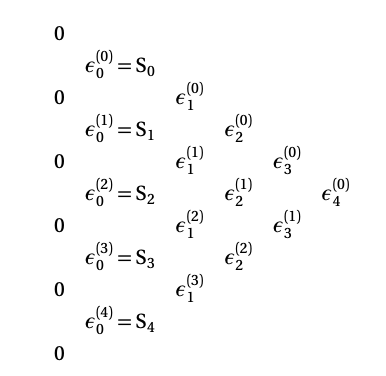
\includegraphics[scale=0.3]{figs/epsilon_tri_array.png}
        \caption{Tableau triangulaire représentant le mode de fonctionnement
        de l'algorithme epsilon pour une série de 5 termes \cite{SENECH}.}
        \label{fig: epsilon_tri_array}
    \end{figure}
    Soit la figure \ref{fig: epsilon_tri_array}, on voit que chaque élément du
    tableau est déterminé grâce aux trois éléments qui figurent en haut à
    gauche, directement à gauche et en bas à gauche jusqu'à arriver au dernier
    élément puisque cela forme un triangle. Numériquement, on initialise
    d'abord la première colonne de valeur comme
    \begin{align*}
        \epsilon_{k=-1}^{(n)} = 0\betspace\epsilon_{k=0}^{(n)} = S_n,
    \end{align*}
    pour ensuite déterminer les autres termes du tableau grâce à l'expression
    \begin{align*}
        \epsilon_{k + 1}^{(n)} = \epsilon_{k - 1}^{(n + 1)} +
        \frac{1}{\epsilon_{k}^{(n + 1)} + \epsilon_{k}^{(n)}}\eqtext{}\forall
        n, k\in\mathbb{N}
    \end{align*}
    où l'on considère qu'il y à $n$ lignes et $k$ colonnes dans le tableau
    triangulaire. On note également que les termes dans les colonnes d'indices
    impairs ne constituent pas de bonnes approximations pour la série $S_n$ et
    donc si l'on donne à l'algorithme une nombre de termes impairs, il est
    impératif d'ajouter une colonne nulle à l'indice $k=-1$ de sorte à ce qu'à
    la fin de l'algorithme la valeur retournée soit précisément celle qui soit
    le pic du triangle.
